\subsubsection{UC19 - Visualizzazione errore validazione file}\label{UC19}

\begin{figure}[H]
  \centering
  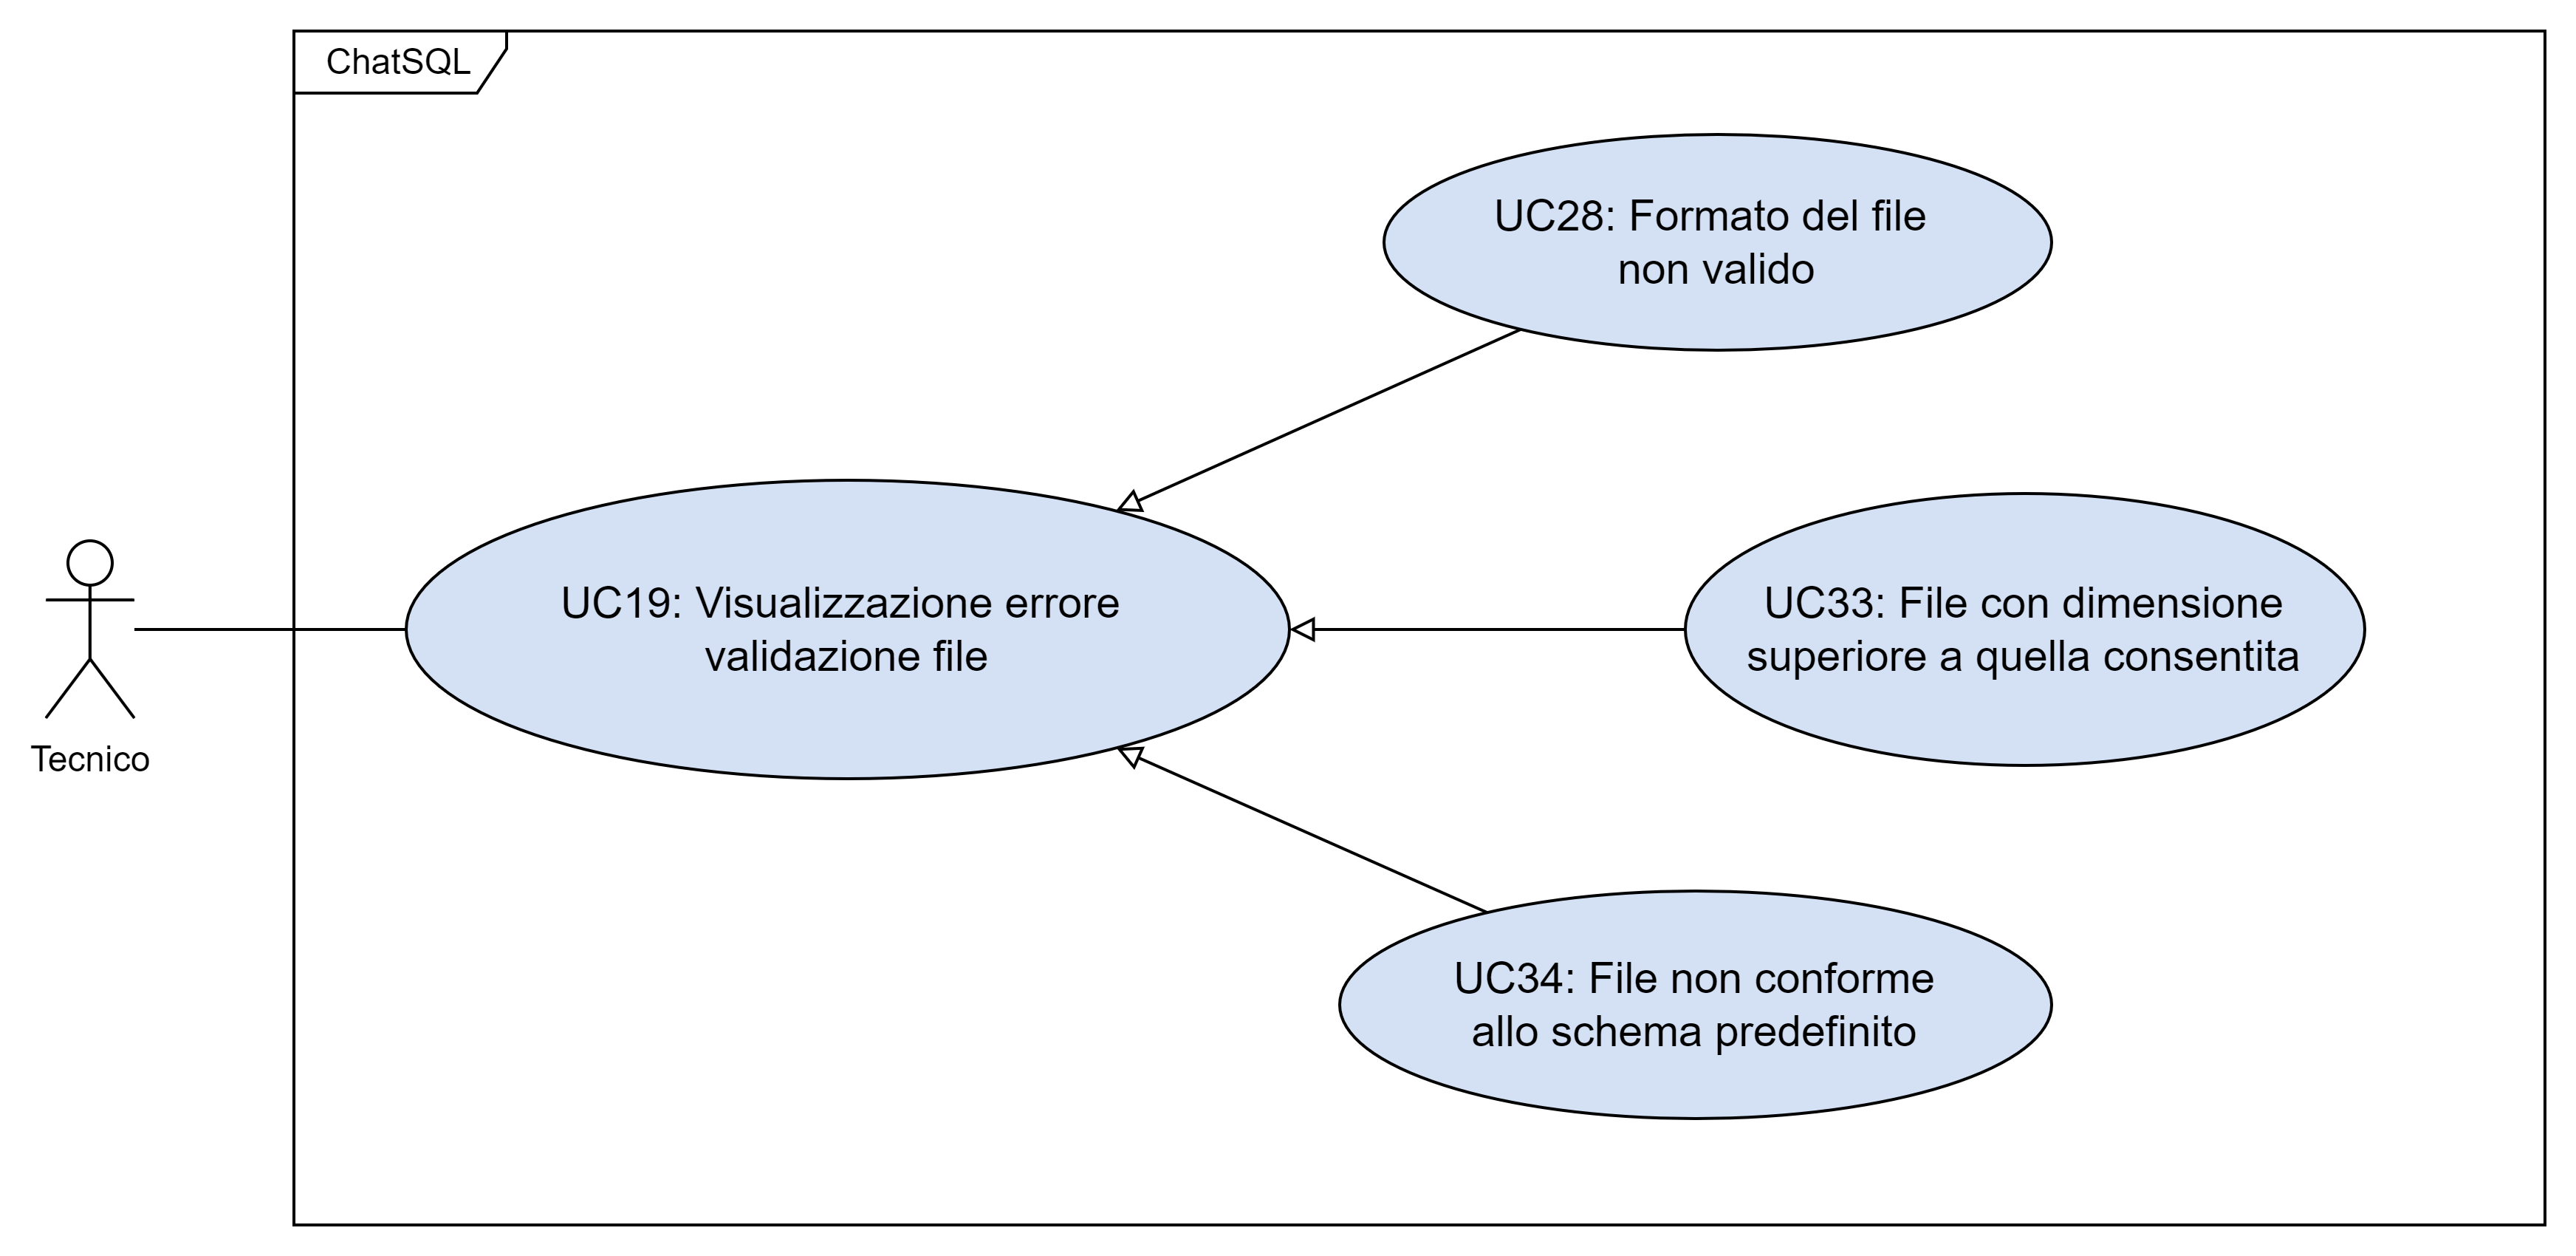
\includegraphics[width=0.90\textwidth]{assets/uc19.png}
  \caption{UC19}
\end{figure}

\paragraph*{Descrizione}
Nel caso in cui il sistema riscontri delle anomalie nella validazione del file scelto come glossario{dizionario dati}, l'Utente visualizza un messaggio d'errore.

\paragraph*{Attori principali}
Tecnico

\paragraph*{Precondizioni}
\begin{itemize}
  \item L'Utente ha richiesto il salvataggio o la modifica di un \glossario{dizionario dati} nel sistema;
  \item Il file caricato non è valido.
\end{itemize}

\paragraph*{Postcondizioni}
\begin{itemize}
  \item Viene mostrato correttamente il messaggio d'errore.
\end{itemize}

\paragraph*{Scenario principale}
\begin{enumerate}
  \item Il sistema riscontra un errore nella validazione del file scelto come \glossario{dizionario dati};
  \item Il sistema restituisce un messaggio con i dettagli dell'errore. 
\end{enumerate}